\documentclass[a4paper,11pt]{article}
\usepackage{a4wide}
\usepackage{amsmath}
\usepackage{amssymb}
\usepackage{amsthm}
\usepackage[ngerman]{babel}
\usepackage{calc}
\usepackage{cancel}
\usepackage{fancyhdr}
\usepackage{float}
\usepackage[margin=1.7cm]{geometry}
\usepackage{graphicx}
\usepackage[utf8]{inputenc}
\usepackage{lastpage}
\usepackage{titlesec}
\usepackage{listings}
\usepackage{stmaryrd}
\usepackage{textpos}
\usepackage{ulem}
\usepackage[usenames,table]{xcolor}
\usepackage{mathtools}
\usepackage[per-mode=fraction]{siunitx}
\usepackage[hyphens]{url}
% make footnote texts have a hanging indentation
\usepackage[hang]{footmisc}


\makeatletter
\let\@addpunct\@gobble
\makeatother
\setcounter{tocdepth}{3}
\newlength{\boxheight}

\sisetup{
    locale=DE,
    detect-all=true,
    quotient-mode=fraction,
    fraction-function=\frac
}
\DeclareSIUnit{\calorie}{cal}

\definecolor{th}{gray}{0.85}
\definecolor{tr-highlighted}{gray}{0.95}

\let\oldemptyset\emptyset
\let\emptyset\varnothing
% See https://tex.stackexchange.com/a/339555
\newdimen{\KernAmount}
\newcommand{\cancelsup}[2]{%
  \setlength{\KernAmount}{\widthof{{\scriptsize \cancel{#1}}}*\real{-1}}%
  #2\kern\KernAmount\vphantom{}^{\cancel{\phantom{#1}}}}
\newcommand{\canceltosup}[3]{%
  \setlength{\KernAmount}{\widthof{{\scriptsize \cancel{#1}}}*\real{-1}}%
  #3\kern\KernAmount\vphantom{}^{\cancel{\phantom{#1}}}\vphantom{}^{^{#2}}}

% See https://en.wikibooks.org/wiki/LaTeX/Source_Code_Listings#Automating_file_inclusion
\newcommand{\includecode}[2][c]{\lstinputlisting[caption=\texttt{#2}, escapechar=, style=custom#1]{#2}}


% make lstlisting floatable and make code look nice
\newfloat{lstfloat}{hp}{lop}
\floatname{lstfloat}{Listing}
\lstset{
  language=Python,
  extendedchars=true,
  literate={ö}{{\"o}}1
    {ä}{{\"a}}1
    {ü}{{\"u}}1
    {Ö}{{\"O}}1
    {Ä}{{\"A}}1
    {Ü}{{\"U}}1,
  basicstyle=\ttfamily\small\upshape,
  commentstyle=\itshape\color{purple!40!black},
  % identifierstyle=\color{blue},
  keywordstyle=\bfseries\color{green!40!black},
  morekeywords={sprintf, usart2_send},
  breaklines=true,
  tabsize=2,
  xleftmargin=3mm,
  xrightmargin=3mm,
  numbers=none,
  frame=single,
  rulesepcolor=\color{gray},
  rulecolor=\color{black},
  stringstyle=\color{orange},
  showstringspaces=false,
}

\newcommand{\image}[4]{\begin{textblock*}{#2 cm}(#3 cm,#4 cm) \includegraphics[width=#2 cm]{#1} \end{textblock*}}
\newcommand\zb{z.\,B.\ }
\newcommand\zt{z.\,T.\ }
\renewcommand\dh{d.\,h.\ }

\newcommand\parbig{\par\bigskip}
\newcommand\parmed{\par\medskip}
\newcommand{\task}[1]{{\parbig\textit{#1}}\\[1mm]}
\newcommand{\taskdesc}[1]{{\parbig#1}}
\newcommand{\names}{Jim Neuendorf, Juri Torhoff}
\newcommand{\protocolnumber}{AB5}

% Header and Footer Style
\pagestyle{fancy}
\fancyhead{}
\fancyhead[C]{\slshape \protocolnumber\;\;--\;\;\names}
\fancyfoot{}
\fancyfoot[C]{\thepage\ von \pageref{LastPage}}

\titlespacing\section{0pt}{20pt}{3pt}
\titlespacing\subsection{0pt}{0pt}{-2pt}

% No identation
\setlength\headheight{15pt}
\setlength\parindent{0pt}

%%%%%%%%%%%%%%%%%%%%%%%%%%%%%%%%%%%%%%%%%%%%%%%%%%%%%%%%%%%%%%%%%%%%%%%%%%%%%%%

\begin{document}

\begin{center}
{\bf \LARGE Maschinelles Lernen}\\[4mm]
\end{center}

\section*{\protocolnumber}
\vspace*{5mm}


\subsection*{\protocolnumber.1 Neuronale Netze und Ziffern}
\task{Implementieren Sie ein neuronales Netz und wenden Sie dieses auf alle Klassen des Digit-Datensatzes an. Um eine bessere Genauigkeit zu erreichen, können Sie anschließend den kompletten Trainingsdatensatz benutzen. Hier müssen ggf. die Merkmale normalisiert werden. Variieren Sie die Anzahl hidden-Layers bzw. Anzahl Neuronen und vergleichen Sie anschließend die Ergebnisse. Plotten Sie wie sich die Klassifikationsgenauigkeit über die Iterationen verändert.}

Bei der Implementierung (siehe unten) gibt scheinbar einen Fehler, da die Konfusionsmatrizen fehlerhaft aussehen.
Egal wie das Netz konfiguriert und trainiert wird, alle Testdaten werden immer auf nur \textit{ein Label} abgebildet, \dh es ist immer nur eine Spalte der Konfusionsmatrizen gefüllt.
Von den rund 7000 Testdaten ergeben ca. höchstens zehn Stück ein anderes Label.
Dadurch ist die Genauigkeit natürlich nur sehr klein (unter $10\,\%$, siehe Plots).

Beim Debuggen bin ich darauf gestoßen, dass ab einer bestimmten Gewichtsmatrix $\overline{W}_i$ in der Kette von Multiplikationen die Output-Vektoren $\overrightarrow{O}_i$ für alle $x_{test} \in X_{test}$ gleich sind.
D.\,h. es gibt folgende Beobachtung:

\begin{align*}
    \hat{O}_i_{x_p} & \neq \hat{O}_i_{x_q} \quad x_p, x_q \in X_{test}\\
    \\
    \text{aber}\\
    \\
    \hat{O}_i_{x_p} \cdot \overline{W}_i & = \hat{O}_i_{x_q} \cdot \overline{W}_i
\end{align*}

Somit sind ab diesem einen $i$ alle Ouputs $\{\overrightarrow{O}_j \, | \, i \leq j \leq L\}\,$\footnote{$L$ ist die Anzahl aller Layer.} für alle $x_{test}$ gleich, \dh auch der finale Output-Vektor.

Ich habe auch versucht die \textit{RELU}- statt der Sigmoidalfunktion benutzen, weil ich dachte, es gibt vielleicht zu kleine Werte, sodass Parameter zu Null werden, aber das hat nichts verändert.\\
\\
Aus diesem Grund wurde der größere Testdatensatz nicht verwendet.\\
% Make footnote go down
\\[7cm]



\pagebreak
Für die Plots der Klassifikationsgenauigkeiten wurden einmal zwei \textit{hidden layers} mit 40 bzw. 50 Elementen (siehe \texttt{main.py}) und ein zweites Mal drei \textit{hidden layers} mit 180, 100 bzw. 50 Elementen verwendet.\\
\\
Beim zweiten Versuch, war die Genauigkeit zwar etwas größer, aber ist trotzdem nicht konvergiert.

\begin{figure}[H]
    \centering
        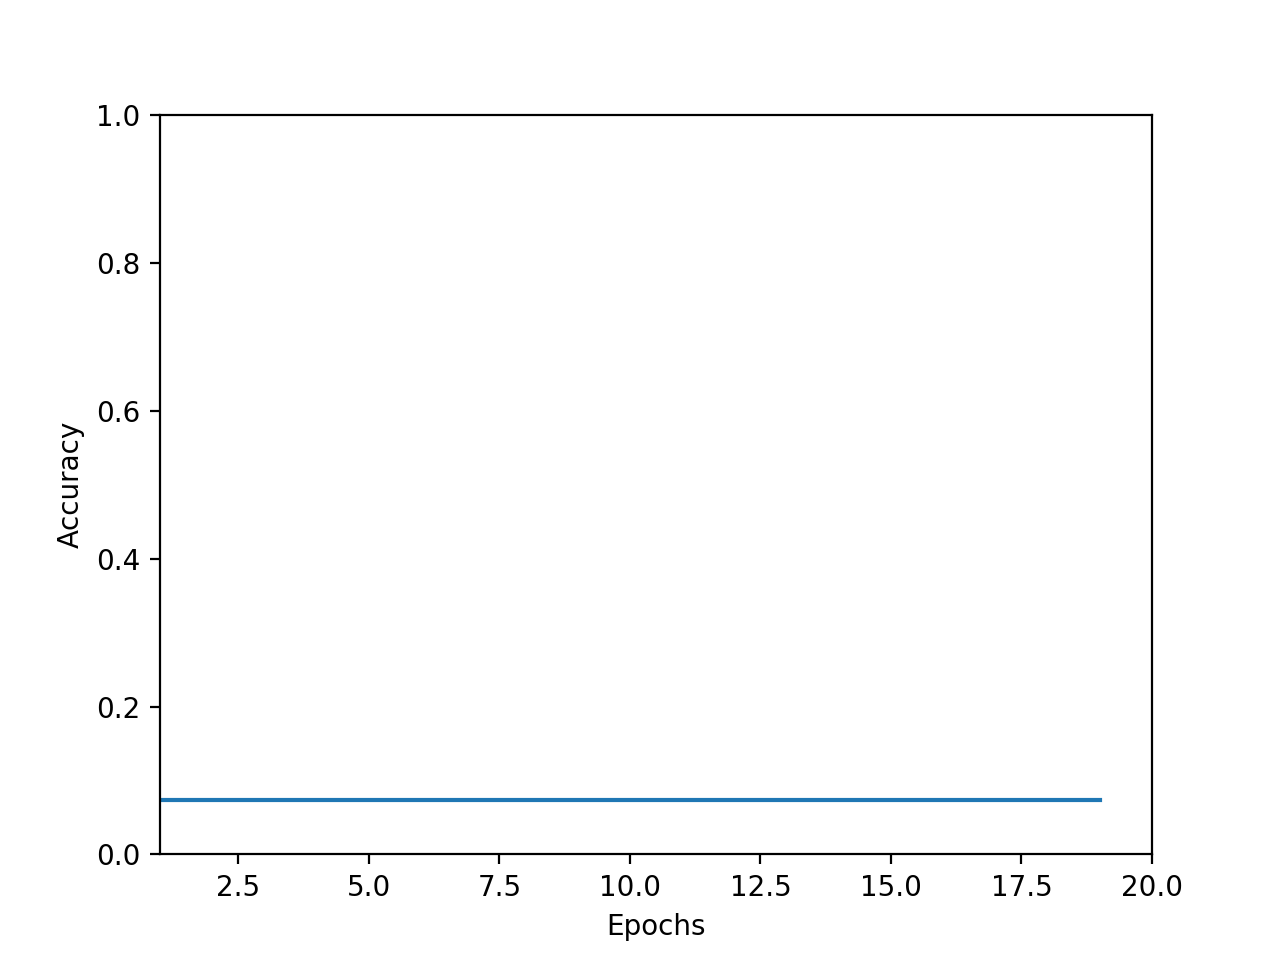
\includegraphics[width=0.75\textwidth]{Figure_1.png}
    \caption{Klassifikationsgenauigkeit pro Anzahl von Epochen für $l = (40, 50)$ und $\gamma = 10^{-3}$}}
\end{figure}
\begin{figure}[H]
    \centering
        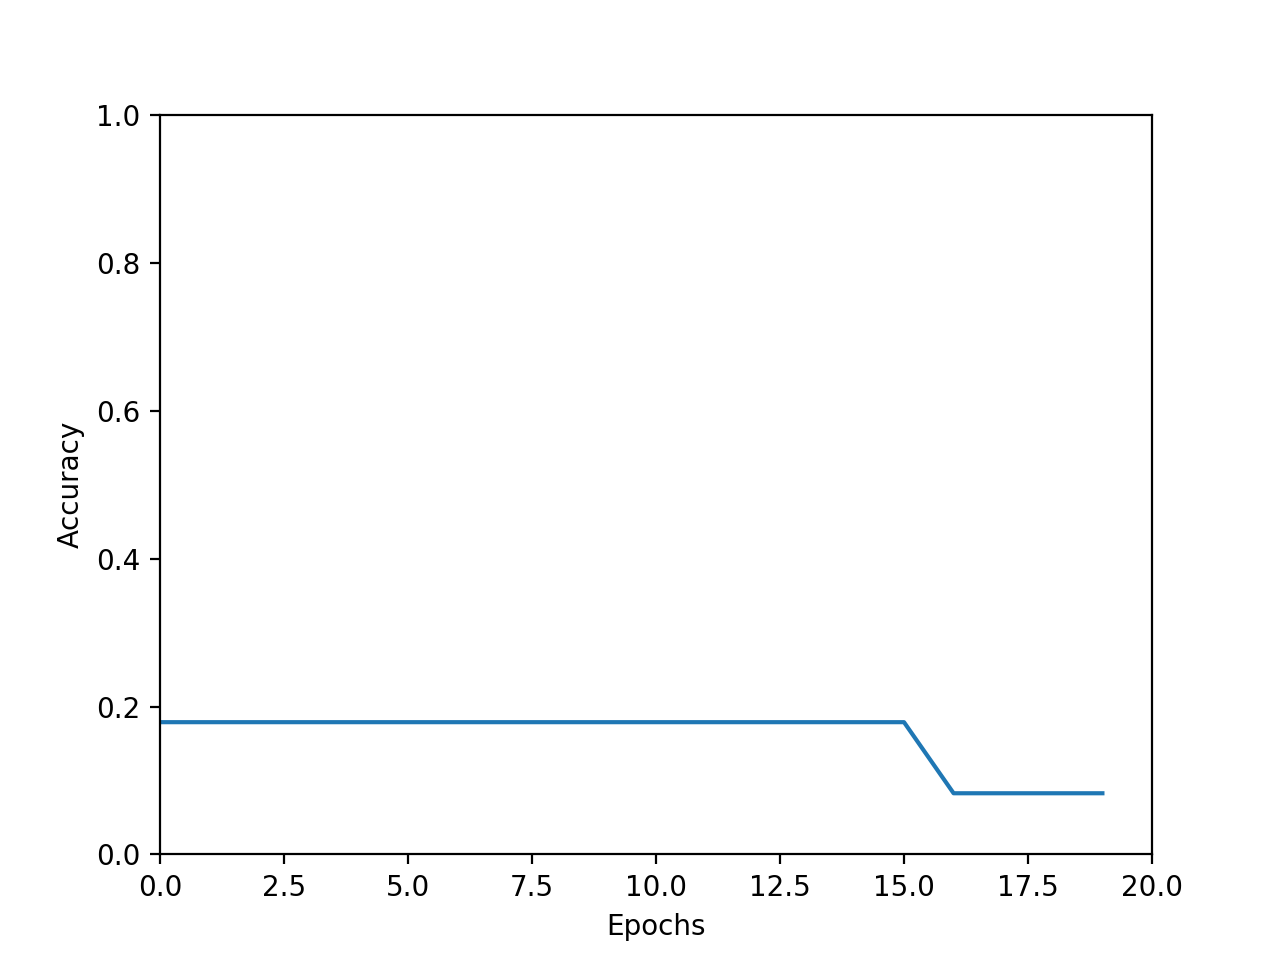
\includegraphics[width=0.75\textwidth]{Figure_2.png}
    \caption{Klassifikationsgenauigkeit pro Anzahl von Epochen für $l = (180, 100, 50)$ und $\gamma = 10^{-5}$}}
\end{figure}



\pagebreak
Das neuronale Netz wurde wie folgt implementiert.

\includecode{src/main.py}

\pagebreak
\includecode{src/classifier.py}

\pagebreak
\includecode{src/neuralnetwork.py}

\pagebreak
\includecode{src/utils.py}


\end{document}
